\section{Learning Outcomes}

\noindent By the end of today's session you will know how to:
\begin{enumerate} 
\item Open a range of different file formats in \texttt{Python}.
\item Use arrays as images, manipulating and plotting them.
\item Compute histograms and plot them.
\item Perform simple fitting on data.
\item Perform simple integration using \texttt{scipy}.
\end{enumerate}

In this chapter we will try to demonstrate some of the uses of \texttt{Python} you will come across in the future, either in modules or research projects. Particularly, in Year 2 you will have a module called Scientific Computing, this module is designed to teach you the theory behind many scientific computing concepts but it \textbf{is not} an applied module, i.e it will not explicitly spell out how to do certain operations. We therefore hope that this chapter will provide a nice introduction to implementing some of these operations. 

As with so much else we have shown you, we don't write out these operations by hand, there are far more capable and knowledgeable people out in the world who have developed packages to perform scientific operations much faster than we ever could. For this we will not only use \texttt{numpy}, which you had an introduction to last chapter, but we will also focus on \texttt{scipy} which (unsurprisingly) stands for scientific python. This module is somewhat like \texttt{numpy}, in that it contains many sub modules for performing many different operations. These include integration, curve fitting, interpolation, signal processing and spatial computations to name a few.

\section{Opening Different File Types}

Regardless of what field you end up specialising in it's certain you'll be handling data in a range of different formats. There are standard formats like text files, \texttt{pickle} files, \texttt{numpy} files, hdf5 files, fits files, and csv files (which you've already seen). There are also a plethora of proprietary formats used in specifics fields for specific functions; for instance the Met Office use a data format modelled after HDF5 files called netCDF4 files which they use specifically for storing weather data.

In this section we will cover the simple formats which you will come across again and again. Hopefully this introduction, and the demonstrations it contains, will mean you will be unfazed when presented with a file to open for an assignment or project in the future.

\subsection{\texttt{with} and the importance of closing files}

One thing which has been seen time and time again is files becoming corrupted due to careless handling. This isn't a big deal for a file which is backed up or can easily be reproduced but in many instances you might be working with a one off file containing terabytes of data which took days, if not weeks or months, to produce. It is therefore very important to learn how to correctly handle data files. The most important thing to remember is if you have opened a file you must close it! Many data files will allow you to do this manually in some way with a function called close. For instance in HDF5 (which we will not cover in great detail here) you can open and close a file like this:

\begin{lstlisting}[style=PY]
In [1]: # Open a file
        hdf = h5py.File('myfile.hdf5', 'r')
        
        # Do some stuff with the contents of the file
        do_stuff(hdf)
        
        hdf.close()
\end{lstlisting}

Doing this safely closes the file, preventing possible corruption from closing improperly. Don't worry about the specifics of the above example, we include it simply as a demonstration of the different methods to open and close files.

The above method is implemented in a number of modules for handling different file formats but how it works is entirely format specific, and also specific to the module being used to handle that format. Thankfully \texttt{Python} includes the \texttt{with} statement structure. This statement will open a file and perform the operations indented below the \texttt{with} declaration before safely closing the file. This is structured in the following manner.

\begin{lstlisting}[style=PY]
In [2]: with file as a:
            do_stuff(a)
\end{lstlisting}

You will see in the following sections the different things that `file' can be replaced with. An important thing to note is that if you simply want to extract the data within a file you can simply assign it to a variable within the {\tt with} statement and the data will be assigned to the variable even after the file has been closed.

\begin{lstlisting}[style=PY]
In [3]: with file as a:  # open file
            x = a.read()  # store data in variable 
        
        # File is closed
        
        # Perform operations on the data that was stored in file
        do_stuff(x)
\end{lstlisting}

Indeed (for completeness) you can combine the HDF5 example with ``\texttt{with}" and can then omit the \texttt{.close()} call.

\begin{lstlisting}[style=PY]
In [4]: with h5py.File('myfile.hdf5', 'r') as a:  # open file
            do_stuff(a) 
        
        # File is closed
\end{lstlisting}

The following sections contain demonstrations of how to open different file types. The examples in these sections will all give errors if you try to run them, since you do not have the files quoted within them.  They are simply provided here for reference.

\subsection{Text and binary files}

With simple text or binary files (these are files which aren't human readable but are saved with strings of binary or hex) we can use the \texttt{Python} open function combined with the \texttt{with} statement. The open function takes a file path as the first argument and a "mode" as the second argument. This mode can be \texttt{'r'} to read a file, \texttt{'w'} to write a file, \texttt{'a'} to append to an existing file or \texttt{'x'} to create a file, the last of these will error if the file already exists. To read a binary file you simply include \texttt{'b'} in the mode, i.e. \texttt{'rb'} to read a binary file.  

\begin{lstlisting}[style=PY]
In [5]: with open('myfile.txt', 'r') as a:
            x = a.read()
\end{lstlisting}

\subsection{Pickle files}

If we have a dictionary and we want to save it the best option is to use a pickle file. This format ``serialises'' the data and can be very efficient when it comes to saving large arrays, not just dictionaries. The extension for a pickle file can effectively be anything (the same is true for binary files) but convention is to use \texttt{.pkl} or \texttt{.pck} which we adopt here.

To use pickle files we need to import the \texttt{pickle} module and call it's \texttt{load} function while using \texttt{open} in binary mode.

\begin{lstlisting}[style=PY]
In [6]: import pickle

        with open('myfile.pck', 'rb') as a:  # open file
            x = pickle.load(a)  # store data in variable 
            
\end{lstlisting}

To save a pickle file we simply exchange \texttt{'rb'} for \texttt{'wb'}, \texttt{load} for \texttt{dump} and provide the variable for saving as the first argument to \texttt{dump} and \texttt{a} as the second.

\begin{lstlisting}[style=PY]
In [7]: import pickle

        with open('myfile.pck', 'wb') as a:  # create file object
            pickle.dump(x, a)  # store data in file
            
\end{lstlisting}

\subsection{\texttt{Numpy} files}

\texttt{Numpy} also provides functions to save and load arrays. These functions do this in nice neat single line statements. In addition to the \texttt{numpy} specific format (\texttt{.npy}) it also has an interface for text files but do be aware that text files will be loaded containing strings rather than floats or integers.

\begin{lstlisting}[style=PY]
In [8]: import numpy as np
        
        # Load a numpy file
        x = np.load('mynumpyfile.npy')
        
        # Load a text file with numpy
        x = np.loadtxt('mytextfile.txt')
        
        # Save a numpy file
        np.save('mynumpyfile.npy', y)
        
        # Save a text file with numpy
        np.savetxt('mytextfile.txt', y)
            
\end{lstlisting}


\begin{tcolorbox}[colback=red!5!white,colframe=red!75!black]
\subsection{FITS files}

FITS (Flexible Image Transport System) files are widely used in astronomy to store images and tabular data. They have a header which contains metadata about the images or tables. The \texttt{astropy} package contains a function for handling these files.

\begin{lstlisting}[style=PY]
In [9]: from astropy.io import fits
        
        # Open the fits file
        hdu = fits.open('myimg.fits')
        
        # Get the first image in the file
        img = hdu[0].data
        
        # Close the file
        hdu.close()
            
\end{lstlisting}

A detailed look at this module and file format can be found here: \url{https://docs.astropy.org/en/stable/io/fits/}.

FITS tables can be read directly into {\tt astropy} tables,
which offer very similar functionality to pandas data frames,
see https://docs.astropy.org/en/stable/table/index.html.

\end{tcolorbox}

\begin{tcolorbox}[colback=red!5!white,colframe=red!75!black]
\subsection{HDF5 files}

HDF5 files are becoming the norm for storing large amounts of data. They are very time and memory efficient allowing a user to access huge datasets without waiting for the entire file to load. They are structured exactly like dictionaries with keys representing "groups"  with datasets and attributes stored within groups. These groups can then also be nested just like a dictionary. To access a HDF5 file we can use the \texttt{h5py} module.

\begin{lstlisting}[style=PY]
In[10]: import h5py
        
        # Open the HDF5 file
        hdf = h5py.File('myfile.hdf5', 'r')
        
        # Open 2 groups
        grp1 = hdf["myfirstgroupkey"]
        grp2 = hdf["mysecondgroupkey"]
        
        # Extract a dataset from group 1
        dset = grp1["thefirstdataset"]
        
        # This can also be done from the root
        dset = hdf["myfirstgroupkey"]["thefirstdataset"]
        
        # Get an attribute from group 2
        at = grp2.attr["thefirstattribute"]
        
        # Again this can be done from the root group
        at = hdf["mysecondgroupkey"].attr["thefirstattribute"]
        
        # Close the file
        hdf.close()
            
\end{lstlisting}

More details on using \texttt{h5py} and the structure of HDF5 files can be found here: \url{http://docs.h5py.org/en/stable/quick.html}.

\end{tcolorbox}

\newpage

\section{Treating Images As Arrays}

In the simplest terms an image is a 2D array of values representing intensity in each pixel. Hopefully the parallel to a 2D \texttt{numpy} array here should immediately come to mind. This means we can manipulate, probe and produce images using many of the processes we have already covered. 

\subsection{Producing images}

To work with images we first need a way to see them. This is where \texttt{matplotlib} comes to the rescue. In addition to the \texttt{plot} and \texttt{scatter} functions you have already seen, there is also a function for plotting images \texttt{imshow}. To use it you simply supply your image as an argument. Lets set up a random 2D array and plot it as an image.

\begin{lstlisting}[style=PY]
In [1]: # Create an iamge of 1000**2 random values
        img = rng.uniform(1, 100, (1000, 1000))
        
        # Plot the image
        plt.imshow(img)
        plt.show()
\end{lstlisting}

The code above will produce the following image.

\begin{figure}[H]
	\centering
	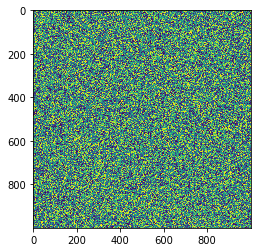
\includegraphics[scale=0.7]{Pictures/randomimgexample.png}
\caption{An image produced from a random uniform distribution.}
\label{fig:randomimg}
\end{figure}

Notice how \texttt{matplotlib} has attributed axis values to the image despite us giving it no information but the x and y ranges. What \texttt{matplotlib} has done is plot the number of pixels along each axis. Let's say we know that the extent of the x and y axes is 200 with the pixels centred on 0 in both axes. We can tell \texttt{matplotlib} this is the case using the \texttt{extent} keyword argument to \texttt{imshow}. 

\newpage

\begin{lstlisting}[style=PY]
In [2]: # Plot the image with an extent
        plt.imshow(img, extent=[-100, 100, -100, 100])

        # Label the axes
        plt.xlabel(r'$x$ (arbitrary units)')
        plt.ylabel(r'$y$ (arbitrary units)')
    
        plt.show()
\end{lstlisting}

The list passed to the \texttt{extent} keyword argument is a list of the extremes along each axis of the form \texttt{[xmin, xmax, ymin, ymax]}. This will then produce the following image.

\begin{figure}[H]
	\centering
	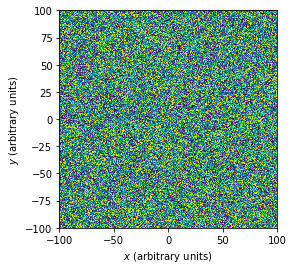
\includegraphics[scale=0.7]{Pictures/randomimgexampleextent.png}
\caption{An image produced from a random uniform distribution showing the use of the \texttt{extent} keyword.}
\label{fig:randimgextent}
\end{figure}

But what if we have an image where we don't want axis labels? In that case you can simply turn off the axes, although there are many ways to do this the simplest is to do the following.

\begin{lstlisting}[style=PY]
In [3]: # Plot the image
        plt.imshow(img)

        # Remove the axes
        plt.axis(False)
        
        plt.show()
\end{lstlisting}

\begin{figure}[H]
	\centering
	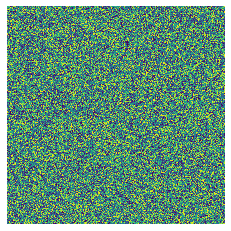
\includegraphics[scale=0.7]{Pictures/randomimgexamplenoaxis.png}
\caption{An image produced from a random uniform distribution with the axes removed.}
\label{fig:randimgnoax}
\end{figure}

The final thing to note is how to apply colormaps. These allow you to make your grayscale images (single values in pixels, rather than RGB arrays with 3 values in each pixel) ``look prettier''. A full list of the available colormaps can be found here: \url{https://matplotlib.org/tutorials/colors/colormaps.html}. To use a colormap you simply supply the name of that colormap to the \texttt{cmap} keyword argument.

\begin{lstlisting}[style=PY]
In [4]: # Plot the image with the plasma colormap
        plt.imshow(img, cmap='plasma')

        # Remove the axes
        plt.axis(False)
        
        plt.show()
\end{lstlisting}

\begin{figure}[H]
	\centering
	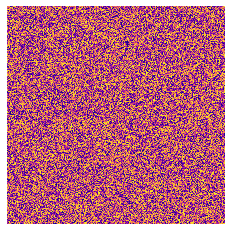
\includegraphics[scale=0.7]{Pictures/randomimgexampleplasma.png}
\caption{An image produced from a random uniform distribution with the plasma colormap.}
\label{fig:randimgnoax}
\end{figure}

\subsection{Manipulating images}
\label{sec:maniimg}

We can treat these images as simple arrays and perform any operation on them that you could on an array. Beyond this however there are a large number of image processing specific modules such as \texttt{PIL}, \texttt{openCV} and \texttt{scikit-image}. We won't go into those here but there's a plethora of image processing possibilities. Here we will just demonstrate some simple operations.

Lets make a more ``interesting" image to do this, a 2D Gaussian. These can be used as an approximation for a poorly resolved point source, or star. To do this we can define a 2D Gaussian function and x and y ranges. From these we can calculate the image with a neat trick to avoid looping.

\begin{lstlisting}[style=PY]
In [5]: # Define a 2D Gaussian function
        def gauss2d(x, y, mx=0, my=0, sigx=1, sigy=1):
            norm = 1. / (2. * np.pi * sigx * sigy)
            exponent = -((x - mx)**2. / (2. * sigx**2.) 
                         + (y - my)**2. / (2. * sigy**2.))
            return norm * np.exp(exponent)
            
        # Define the x and y values
        xs = np.linspace(-5, 5, 1000)
        ys = np.linspace(-5, 5, 1000)
        
        # Combine the x and y ranges into a 2d grid (this is the neat trick)
        xx, yy = np.meshgrid(xs, ys)
        
        # Compute the gaussian image leaving the default values of 0 for the 
        # means and 1 for the standard deviations
        img = gauss2d(xx, yy)
        
        # Plot the image with the known extent and inferno colormap
        plt.imshow(img, extent=[-5, 5, -5, 5], cmap='inferno')

        # Label axes
        plt.xlabel(r'$x$ (arbitrary units)')
        plt.ylabel(r'$y$ (arbitrary units)')
        
        plt.show()
\end{lstlisting}

\begin{figure}[H]
	\centering
	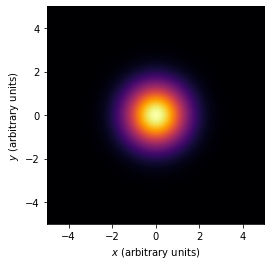
\includegraphics[scale=0.7]{Pictures/gaussimgexample.png}
\caption{An image of a basic 2D Gaussian.}
\label{fig:randimgnoax}
\end{figure}

We can obviously do simple calculations on the image to scale it in different ways but you can play around with that yourself. A more useful function to apply is the base 10 logarithm, this can be very useful for bringing out detail in pictures where a bright set of pixels dominates the image.

\begin{lstlisting}[style=PY]
In [6]: # Scale the image logarithmically
        logimg = np.log10(img)
        
        # Plot the image with the known extent and inferno colormap
        plt.imshow(logimg, extent=[-5, 5, -5, 5], cmap='inferno')

        # Label axes
        plt.xlabel(r'$x$ (arbitrary units)')
        plt.ylabel(r'$y$ (arbitrary units)')
        
        plt.show()
\end{lstlisting}

\begin{figure}[H]
	\centering
	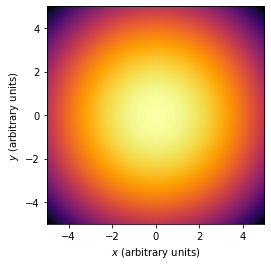
\includegraphics[scale=0.7]{Pictures/gaussimgexamplelog.png}
\caption{An image of a basic 2D Gaussian with logarithmic scaling.}
\label{fig:randimgnoax}
\end{figure}

We can also apply Boolean conditions to control specific regions in the image. Lets remove the background, to do this we can simply define an intensity threshold below which we set the pixel values to \texttt{np.nan}, \texttt{matplotlib} will then interpret these values as transparent.

\begin{lstlisting}[style=PY]
In [7]: # Set any values below 10% of the maximum of the image to be 
        # transparent
        trans_img = img.copy()
        trans_img[img < img.max() * 0.1] = np.nan
        
        # Plot the image with the known extent and inferno colormap
        plt.imshow(trans_img, extent=[-5, 5, -5, 5], cmap='inferno')
        
        # Label axes
        plt.xlabel(r'$x$ (arbitrary units)')
        plt.ylabel(r'$y$ (arbitrary units)')

        plt.show()
\end{lstlisting}

\begin{figure}[H]
	\centering
	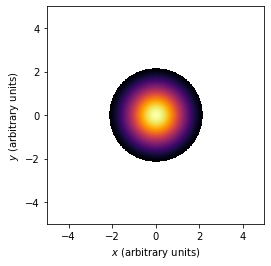
\includegraphics[scale=0.7]{Pictures/gaussimgexampletransparent.png}
\caption{An image of a basic 2D Gaussian with a transparent background.}
\label{fig:randimgnoax}
\end{figure}

One final operation to consider, although it's not of much use here, is the clipping of an image between minimum and maximum intensity values. This will set any values below the minimum to the minimum and any values above the maximum to the maximum. This can be done a number of ways but the simplest is applying a minimum and maximum with \texttt{vmin} and \texttt{vmax}.

\begin{lstlisting}[style=PY]
In [8]: # Plot the image with the known extent and inferno colormap, 
        # setting minimum and maximum intensities
        plt.imshow(img, extent=[-5, 5, -5, 5], cmap='inferno', 
                   vmin=img.max()*0.5, vmax=img.max()*0.8)
        
        # Label axes
        plt.xlabel(r'$x$ (arbitrary units)')
        plt.ylabel(r'$y$ (arbitrary units)')

        plt.show()
\end{lstlisting}

\begin{figure}[H]
	\centering
	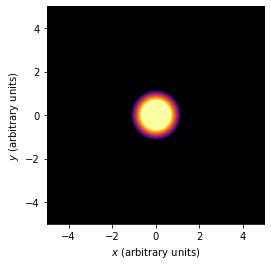
\includegraphics[scale=0.7]{Pictures/gaussimgexamplevmin.png}
\caption{An image of a basic 2D Gaussian with intensities clipped to minimum and maximum values.}
\label{fig:randimgnoax}
\end{figure}

\subsection{Exercises (with worked solutions)} \label{sec:exc_hubble}

We can now apply this to some exercises with a more interesting image.

\begin{enumerate}
\item Download from canvas and open the \texttt{pickle} file ``Hubbleimg.pck" assign the contents to a variable. Plot the image contained in the file. You shouldn't see anything in the image as this is a raw image with minimal processing. This is an image of the pillars of creation taken using the Hubble Space Telescope, although you wouldn't know that at this point.
\item Try scaling the image with different mathematical functions to bring out detail and plot your tests. (Hint: log10 scaling is a good start but there are many many possibilities, have a play).
\item Use \texttt{vmin} and \texttt{vmax} to improve the quality of your image and bring out the maximum detail possible.
\item (No solution) Making these images look good is more art than science. Try to make the best image possible by applying anything you can think of to help. (Hint: You might be able to reduce noise by subtracting the mean or median and re-normalising the values, or maybe there's different scaling you could apply, maybe even look into \texttt{PIL} at the image processing possible with it).
\end{enumerate}

\newpage

\section{Histograms}

In previous exercises (mostly advanced exercises) we have asked you to create histograms as with a bit of brute force it's easy enough to code one up using dictionaries or lists. This said, they are a very powerful analysis tool and come up again and again when analysing data, in fact you should have come across them in labs. To make a histogram you need to sort data into a set of bins. In \texttt{Python} there are a number of ways to produce histograms, we will show the \texttt{numpy} method, there is nothing wrong with any other method and the \texttt{matplotlib} method is similar and produces a plot at the same time, \texttt{numpy} just provides a bit more flexibility before plotting.

To produce a histogram we first need some data to histogram, for this we can just produce random values from a normal distribution, and we need bins in which to sort it. To begin with we can just tell \texttt{numpy} that we want a certain number of bins, a good rule of thumb if you don't explicitly know how many bins you need is to use the square root of the number of data points you have.

\begin{lstlisting}[style=PY]
In [2]: # Define an array of values to histogram
        vals = rng.normal(0, 10, 10000)
        
        # Compute the number of bins (this must be an integer)
        nbin = int(np.sqrt(vals.size))
        
        # Compute the histogram 
        H, bin_edges = np.histogram(vals, bins=nbin)
\end{lstlisting}

We now have the values sorted into bins where \texttt{H} is the number of counts in each bin and \texttt{bin\_edges} is, unsurprisingly, the edges of the bins. These variable names are convention, you can obviously change these. Lets plot these results as a bar graph using \texttt{bar}.

\begin{lstlisting}[style=PY]
In [2]: # Plot the histogram as a bar graph
        plt.bar(bin_edges, H)
        plt.show()
\end{lstlisting}

Of course, you may have seen this coming... but we have an error, specifically ``\texttt{ValueError: shape mismatch: objects cannot be broadcast to a single shape}'. This is because \texttt{H} and \texttt{bin\_edges} are different sizes because \texttt{bin\_edges} contains the edges of the bins, i.e. 1 more entry than \texttt{H}. We want to plot against the centre of each bin. Not to worry though, this is easily achieved.

\begin{lstlisting}[style=PY]
In [2]: # Compute the bin centres
        bin_width = bin_edges[1] - bin_edges[0]
        bin_cents = bin_edges[1:] - (bin_width / 2)
        
        # Plot the histogram as a bar graph
        plt.bar(bin_cents, H)
        
        # Label axes
        plt.xlabel(r'$x$')
        plt.ylabel(r'$N$')
        
        plt.show()
\end{lstlisting}

Running the above code produces the plot below (although yours will look subtly different due to the nature of unseeded random numbers). Notice how simply by histograming the values we have roughly reproduced the normal distribution the values were pulled from.

\begin{figure}[H]
	\centering
	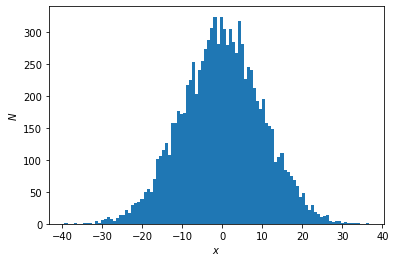
\includegraphics[scale=0.7]{Pictures/histexample.png}
\caption{An example histogram of values pulled from a normal distribution.}
\label{fig:randimgnoax}
\end{figure}

Another way to achieve the same result is by defining the bins ahead of time, this gives the histogram an explict range.

\begin{lstlisting}[style=PY]
In [2]: # Define an array of values to histogram
        vals = rng.normal(0, 10, 10000)
        
        # Compute the number of bins (this must be an integer)
        nbin = int(np.sqrt(vals.size))
        bins = np.linspace(-40, 40, nbin)
        
        # Compute the histogram 
        H, bin_edges = np.histogram(vals, bins=bins)
\end{lstlisting}

We can also produce 2D histograms which are themselves just images, think of a camera collecting photons (counts) in pixels (bins). We can approximate the Gaussian distribution from Sec.\ref{sec:maniimg} very simply by creating a 2D histogram in the same way we just produced a 1-dimensional histogram. Here we will set the number of bins as we did originally (this will apply along both axes) and also define a range for the bins to cover, this is similar to providing an array of bins but instead defines the range in which you put \texttt{nbin} bins, in a similar manner to defining the extent of an image in \texttt{imshow}.

\newpage

\begin{lstlisting}[style=PY]
In [2]: # Define the x and y values from a normal distribution
        xs = rng.normal(0, 1, 100000)
        ys = rng.normal(0, 1, 100000)
        
        # Define the number of bins
        nbin = 100
        
        # Define the range for the bins
        binrange = ((-5, 5), (-5, 5))
        
        # Compute the histogram using the range
        H, xbin_edges, ybin_edges = np.histogram2d(xs, ys, bins=nbin, 
                                                   range=binrange)
        
        # Plot the image
        plt.imshow(H, cmap='viridis', extent=[-5, 5, -5, 5])
        
        # Label axes
        plt.xlabel(r'$x$')
        plt.ylabel(r'$y$')
        
        plt.show()
\end{lstlisting}

\begin{figure}[H]
	\centering
	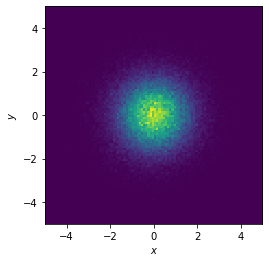
\includegraphics[scale=0.7]{Pictures/hist2dexample.png}
\caption{A 2D Gaussian distribution produced using a 2D histogram.}
\label{fig:randimgnoax}
\end{figure}

This can be very useful for creating images from 1D spatial data. 

\newpage

\section{Basic Curve Fitting}

As you no doubt have already seen, when working with scientific data you're often fitting your experimental data to a model or theory. You can then compute statistics to determine the validity of any theories you may be comparing to. Although you can do this in excel with \texttt{LINEST}, this is very limited both in implementation and in the logistics of working with large data sets. Instead we want to utilise \texttt{scipy.optimize} which contains a fitting function called \texttt{curve\_fit}. Here we will demonstrate how to use \texttt{curve\_fit} so that your ready when you need to use it.

First download the file \texttt{curvefitting.txt} from canvas. We will load this data into your notebook and then fit it with a straight line. To use \texttt{curve\_fit} we need 3 things, the data, a function with the first argument being the x values and any other parameters as the subsequent arguments, and an initial guesses for each of the parameters. Once we have these set up we can call \texttt{curve\_fit} and use the produced parameters to plot the fit.

\begin{lstlisting}[style=PY]
In [2]: from scipy.optimize import curve_fit

        # Load the data
        arr = np.loadtxt('curvefitting.txt')
        
        # Convert the data from strings to floats
        arr = np.float64(arr)
        
        # Extract the xs and ys from the file
        xs = arr[:, 0]
        ys = arr[:, 1]
        
        # Define a function to fit the data to
        def func(x, m, c):
            return m * x + c
        
        # Define some initial guesses for m and c
        guesses = [1, 1]
        
        # Get the fit
        popt, pcov = curve_fit(func, xs, ys, p0=guesses)
        
        # Compute the fit using the parameters in popt
        fit = func(xs, popt[0], popt[1])
        
        # Plot the resulting fit and data
        plt.scatter(xs, ys, marker='+')
        plt.plot(xs, fit, linestyle='--')
        
        # Label axes
        plt.xlabel(r'$x$')
        plt.ylabel(r'$y$')
        
        plt.show()
\end{lstlisting}

There are a few things to note in the code snippet above. Firstly, when opening a text file the contents within will have been converted to strings, to deal with this we have used \texttt{np.float64} to convert the array into 64-bit floats. Secondly, the data is stored in a (100, 2) array with the xs in the first column and the ys in the second column, we have had to use slicing to extract these into their own arrays. 

On the topic of the guesses, \texttt{curve\_fit} is fairly capable of handling even bad guesses so anything in the ball park of the right values should suffice. If you provide guesses miles from the truth it is possible for the fitting to fail, try it and see what happens. Finally, take a look at what is returned by \texttt{curve\_fit}, \texttt{popt} contains the optimal parameters in the same order they appear in the arguments of the function, \texttt{pcov} on the other hand is the covariance matrix, this is a concept from statistics which you will come across in the future so we will skirt around the complexities but it is enough right now to say the diagonal elements of \texttt{pcov} are the uncertainties on the returned parameters.

\begin{figure}[H]
	\centering
	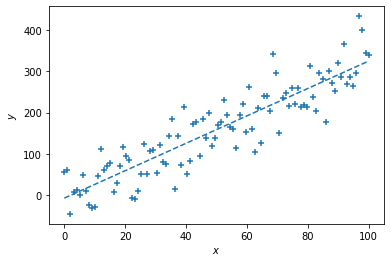
\includegraphics[scale=0.7]{Pictures/fittingexample.png}
\caption{A plot of the fit produced using \texttt{curve\_fit}.}
\label{fig:randimgnoax}
\end{figure}

Hopefully this serves as a brief introduction to using \texttt{curve\_fit} and it won't cause you distress when you come across it in the future. We will cover another example in the exercises.

\newpage

\section{Integration}

Another staple in scientific computing is the numerical computation of integrals, with some integrals not having analytical solutions at all. You may have come across ways to approximate integrals in the past such as the trapezium and Simpson's rules. There are multiple implementations of these from different modules, here we will cover \texttt{scipy} but do note that these functions can be used in a number of ways, either providing x values or an interval $dx$ at which to calculate the integration. 

To compute an integral with these functions we will define two arrays one of x values and one containing the result from a 1D Gaussian, normalised such that the integral should be unity. We can then apply the functions and see if we sampled with fine enough resolution to get the expected result.

\begin{lstlisting}[style=PY]
In [2]: from scipy.integrate import simps, trapz

        # Define some xs
        xs = np.linspace(-50, 50, 1000)
        
        # Define a 1D Gaussian function
        def gauss(x, mx=0, sigx=1):
            norm = 1. / np.sqrt(2. * np.pi * sigx**2)
            exponent = - (x - mx)**2. / (2. * sigx**2.)
            return norm * np.exp(exponent)
        
        # Compute the Gaussian
        ys = gauss(xs)
        
        # Compute the integral by the trapezium and Simpson's rule 
        trap = trapz(ys, xs)
        simp = simps(ys, xs)
        
        print(trap, simp)
\end{lstlisting}
\begin{lstlisting}[style=PY, backgroundcolor=\color{white}]
        1.0 1.0
\end{lstlisting}

Evidently in both case we did sample with high enough resolution and over a large enough range. That said, for such a simple function this shouldn't be a surprise.

\newpage

In addition to the trapezium and Simpson's rules \texttt{scipy} also contains a function called \texttt{quad} which allows you to compute integrals from a function. Let's reproduce the above example but using \texttt{quad}. To use \texttt{quad} we need to define a 1D Gaussian as a function and define upper ($b$) and lower ($a$) bounds for the integration.

\begin{lstlisting}[style=PY]
In [2]: from scipy.integrate import quad

        # Define some xs
        xs = np.linspace(-5, 5, 1000)
        
        # Define a 1D Gaussian function
        def gauss(x, mx=0, sigx=1):
            norm = 1. / np.sqrt(2. * np.pi * sigx**2)
            exponent = - (x - mx)**2. / (2. * sigx**2.)
            return norm * np.exp(exponent)
        
        # Compute the integral by the trapezium and simpsons rule 
        qu = quad(gauss, a=-50, b=50)

        print(qu)
\end{lstlisting}
\begin{lstlisting}[style=PY, backgroundcolor=\color{white}]
        (1.0000000000000002, 1.0346447325665705e-12)
\end{lstlisting}

At first glance \texttt{quad} didn't give as perfect a result as the simpler methods above, however one nice thing about \texttt{quad} is it also computes an error on the integration. Taking this error into account the result is indeed consistent with the expected result of unity. The inclusion of an error makes \texttt{quad} very useful and as functions get more complex \texttt{quad} really begins to shine. 

We have not covered the entirety of the possible integration methods provided by \texttt{scipy}, for a full list and a tutorial see \url{https://docs.scipy.org/doc/scipy/reference/tutorial/integrate.html}.

\subsection{Exercises (with worked solutions)} \label{sec:exc_integration}

\begin{enumerate}
\item Generate the 1D Gaussian from the examples in the histogram section but this time taking only 1000 values.
\item Create a histogram of the random samples.
\item Define a Gaussian function and fit it. Plot the resulting histogram and fit as a bar plot and dashed line respectively. (Hint: you can make the normalisation a fitting parameter as well).
\item Integrate $\sin^2(x)\cos^3(x)$ and $\sin^2(x)\cos^4(x)$ between $-2\pi$ and $2\pi$. Before you calculate them do you know immediately which should be 0? There's a hidden integration trick here with multiplying odd and even functions when combined with symmetric limits.
\end{enumerate}

\newpage

\section{Worked Solutions}
\textbf{\ref{sec:exc_hubble}}

\begin{lstlisting}[style=PY]
In [1]: import pickle
        import matplotlib.pyplot as plt
        import numpy as np
        
        # Question 1
        
        with open("Hubbleimg.pck", 'rb')as pfile:
            img = pickle.load(pfile)
        
        # Plot raw image
        plt.imshow(img, cmap='Greys_r')
        plt.axis(False)
        plt.show()
\end{lstlisting}

\begin{figure}[H]
	\centering
	
\includegraphics[scale=1.2]{Pictures/rawimg.png}
\end{figure}

\newpage

\begin{lstlisting}[style=PY]
In [2]: # Question 2
        # Scale the image to better show detail
        logimg = np.log10(img)
        asinimg = np.arcsinh(img)
        
        # Plot each image
        plt.imshow(logimg, cmap='Greys_r')
        # NOTE: log10 produces some -inf where there are 0 counts, 
        # hence the error
        plt.title("Log scaling")
        plt.axis(False)
        plt.show()
        plt.imshow(asinimg, cmap='Greys_r')
        plt.title("Arcsinh scaling")
        plt.axis(False)
        plt.show()
\end{lstlisting}

\begin{figure}[H]
	\centering
	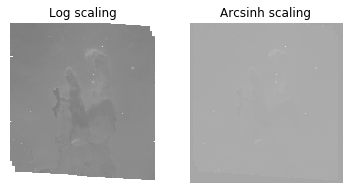
\includegraphics[width=\linewidth]{Pictures/logasinimg.png}
\end{figure}

\newpage

\begin{lstlisting}[style=PY]
In [3]: # Question 3
        # Find minima and maxima counts that correspond to detail in 
        # the nebula
        print(np.min(logimg[np.logical_and(logimg != -np.inf, 
                                           ~np.isnan(logimg))]))
        print(np.min(asinimg))
        print(np.max(logimg[~np.isnan(logimg)]))
        print(np.max(asinimg))
        
        # Plot the image setting the minimum value and maximum
        plt.imshow(logimg, cmap='Greys_r', vmin=-1.5, vmax=0.5) 
        plt.title("Log scaling Clipped")
        plt.axis(False)
        plt.show()
        plt.imshow(asinimg, cmap='Greys_r', vmin=-0.1, vmax=0.75)
        plt.title("Arcsinh scaling Clipped")
        plt.axis(False)
        plt.show()
        
        # We can permenantly apply these changes to the images using np.clip
        logimg = np.clip(logimg, a_min=-1.5, a_max=0.5) 
        asinimg = np.clip(asinimg, a_min=-0.1, a_max=0.75)
        
        # NOTE: these values aren't "correct" (neither are the choices of 
        # scalings the only possible choices) they are the values chosen 
        # while doing this worked example. There almost certainly are 
        # better combinations!
\end{lstlisting}

\begin{figure}[H]
	\centering
	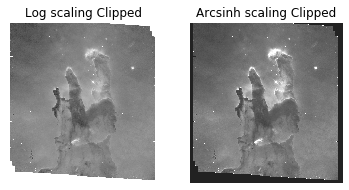
\includegraphics[width=\linewidth]{Pictures/logasinimgnormed.png}
\end{figure}

\newpage

\textbf{\ref{sec:exc_integration}}

\begin{lstlisting}[style=PY]
In [1]: import numpy as np
        import matplotlib.pyplot as plt
        from scipy.integrate import quad
        from scipy.optimize import curve_fit
        
        # Question 1
        # Define an array of values to histogram
        vals = rng.normal(0, 10, 1000)
        
        
        # Question 2
        # Compute the number of bins 
        nbin = int(np.sqrt(vals.size))
        
        # Compute the histogram 
        H, bin_edges = np.histogram(vals, bins=nbin)
        
        # Question 3
        # Define a 1D Gaussian function
        def gauss(x, norm, mx, sigx):
            exponent = - (x - mx)**2. / (2. * sigx**2.)
            return norm * np.exp(exponent)
        
        # Define guesses for the gaussian parameters
        guesses = [100, 0, 10]

        # Compute the bin centres
        bin_width = bin_edges[1] - bin_edges[0]
        bin_cents = bin_edges[1:] - (bin_width / 2)
        
        # Get the fitting parameters
        popt, pcov = curve_fit(gauss, bin_cents, H, p0=guesses)
        
        print('Fit parameters are:', popt)
        
        # Evaluate the fit
        fit_xs = np.linspace(-50, 50, 10000)
        fit = gauss(fit_xs, popt[0], popt[1], popt[2])
        
        # Plot the histogram as a bar graph
        plt.bar(bin_cents, H, width=bin_width, alpha=0.8, edgecolor='k')
        plt.plot(fit_xs, fit, linestyle='--', color='r', linewidth=4)
        
        # Label axes
        plt.xlabel(r'$x$')
        plt.ylabel(r'$N$')
        
        plt.show()
\end{lstlisting}

\begin{figure}[H]
	\centering
	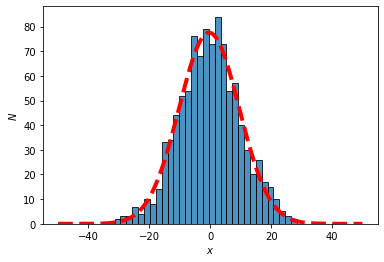
\includegraphics[scale=0.9]{Pictures/histfit.png}
\end{figure}

\begin{lstlisting}[style=PY]
In [2]: # Question 4

        # It's np.sin(x)**2*np.cos(x)**3 which should be 0 as this is an 
        # odd function (cos^3) multiplied by an even function (sin^2) 
        # which results in an odd function, the integral of any odd function 
        # over limits symmetric about 0 is NECESSARILY 0!
        
        # Evaluate integrals defining functions as lambda functions 
        # for neatness
        qu1 = quad(lambda x: np.sin(x)**2*np.cos(x)**3, -2*np.pi, 2*np.pi)
        qu2 = quad(lambda x: np.sin(x)**2*np.cos(x)**4, -2*np.pi, 2*np.pi)
        
        # Print result
        print(qu1)
        print(qu2)
\end{lstlisting}
